\documentclass[a4paper]{jpconf}
\usepackage{graphicx}
\begin{document}
\title{Centre for High Performance Computing Tier2 Facility for WLCG}

\author{Sean Murray}

\address{Center for High Performance Computing\\ CSIR. \\Rosebank \\Cape Town\\7700}

\ead{murrays@cern.ch}

\begin{abstract}

The Worldwide LHC Computing Grid (WLCG) provides computing resources to the four experiments at CERN’s Large Hadron Collider (LHC).  The Centre for High Performance Computing (C.H.P.C) is the only South African Tier-2 centre in the WLCG.

The site currently supplies resources for ALICE and ATLAS in the form of computing, storage and network bandwidth. We will show the current site configuration and performance specifications, plans for the coming year to speed up the work of local South African users and the required deliverables as a Tier-2 centre for the WLCG.
\end{abstract}

\section{Introduction}

The WLCG project is a collaboration of over 170 computing centres in 42 countries, linking national and international grid infrastructures.
It exists provide the necessary computing resources to store, distribute and analyse the data generated by the LHC at CERN.\cite{http://wlcg.web.cern.ch/}
The C.H.P.C. joined the collaboration on 28 April 2015 after signing the Memorandum Of Understanding as a Tier 2 site. 
\begin{figure}[h]
    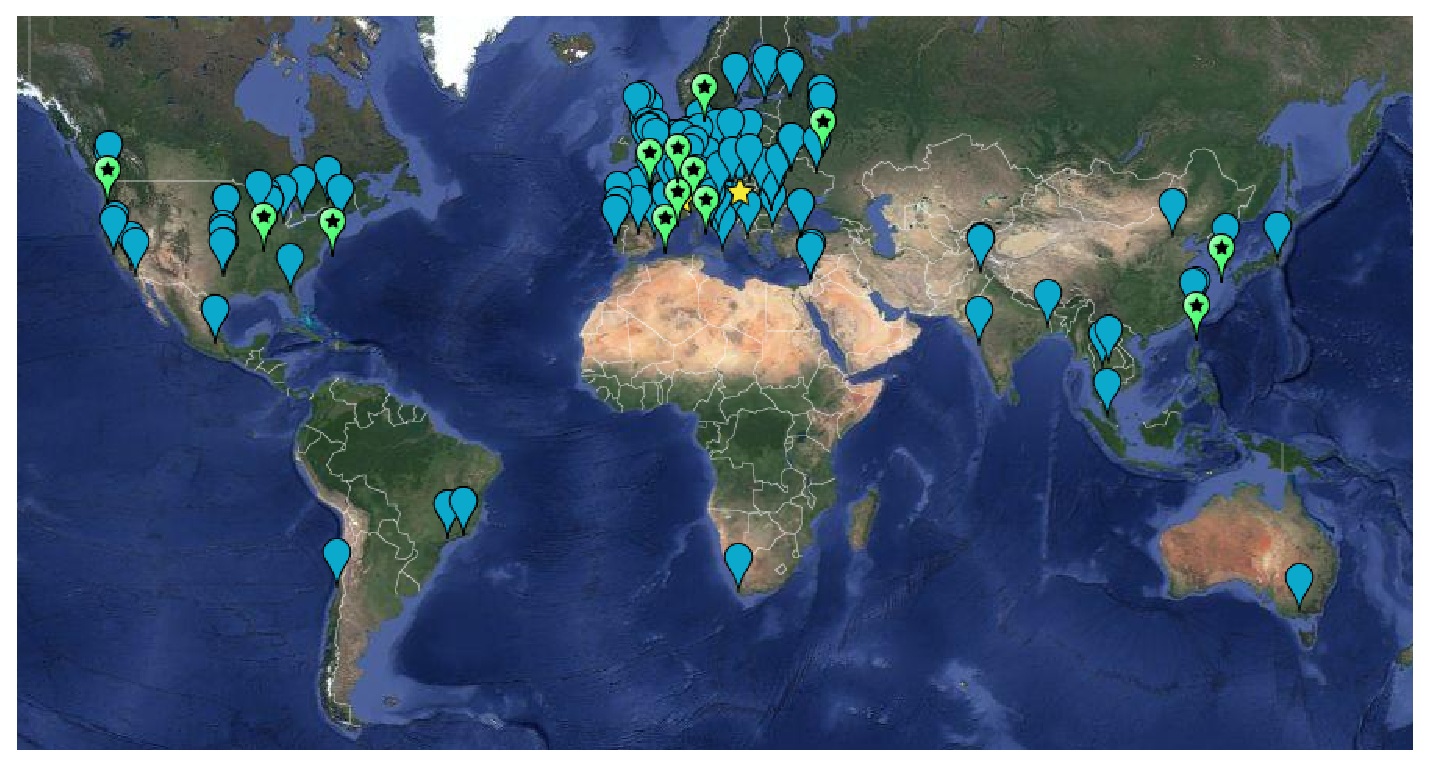
\includegraphics[width=38pc]{WLCG-Sites.eps}
    \caption{\label{label} World map showing all the Tier1 (green) and Tier2 (blue) WLCG sites.}
\end{figure}


\section{Infrastructure}
The current computing infrastructure dedicated to the Tier2 operations is made up of :
\begin{itemize}
  \item 50 nodes of 48 threads, 192GB RAM, 1.6TB SSD local storage, dual 1Gbps ethernet connection
  \item 704TB 10Gbps attached xrootd storage, 400 ALICE, 304 ATLAS.
  \item 8 management nodes, provision, monitoring, authentication, storage1, storage2, compute element, bdii, vobox.
  \item redundant 10Gbps switched backbone.
\end{itemize}
This then satisfies union of minimum computing requirements of ALICE  and ATLAS, which together impose a 
4GB memory requirement per job (ALICE) and 30GB of local storage (ATLAS).
Additionally for wider grid based usage the follow resources are available :
\begin{itemize}
  \item 34 nodes of 48 threads, 96GB RAM, 1TB SATA local storage, FDR infiniband.
  \item 107TB Lustre file system, infiniband connected, shared into the nodes.
  \item 1 management node.
\end{itemize}
The memory of the second set of nodes is less than that of the Tier2 nodes.


\section{Commitments}
ALICE and ATLAS operate slightly differently with regards to resources allocated to the experiments.
ALICE uses a fair share approach based on the number of scientists in the experiment. ATLAS has a specific resource requirement for something to be 
defined as a Tier2.
\begin{table}[h]
  \caption{\label{ex}MOU resource commitments.}
  \begin{center}
    \begin{tabular}{llll}
      \br
      Experiment & CPU [HEP-SPEC06] & Disk [TB] & Disk deficit [TB] \\
      \mr
      ALICE&6000 & 600 & 252\\
      ATLAS&6000 & 600 & 342\\
      \br
    \end{tabular}
  \end{center}
\end{table}
The alignment of ALICE and ATLAS storage, while convenient for us, is completely coincidental, ALICE and ATLAS do their accounting differently. ATLAS has a predefined
specification for a Tier2 facility and this is defined at 600TB of storage, ALICE uses a system based on proportional representation. It is of course convenient for us 
that the numbers are both 600, but this is coincidental. It is however our plan to try and keep our commitments equal to each experiment.


\section{Operation}
The operations delivered are :
\begin{itemize}
  \item ALICE 485 000 jobs in the last year.
  \item Average concurrent job count for the year is 704, including all down time.
  \item ATLAS nominal jobs as they are still sending pilot jobs till the storage is live.
  \item Data transfer, 70TB in and 68TB out in the last 3 months, averaging 100Mbps in and out.
  \item ALICE storage went live, after prolonged testing, on 24 June. It currently holds 7.5TB of output in that 3 weeks.
\end{itemize}
%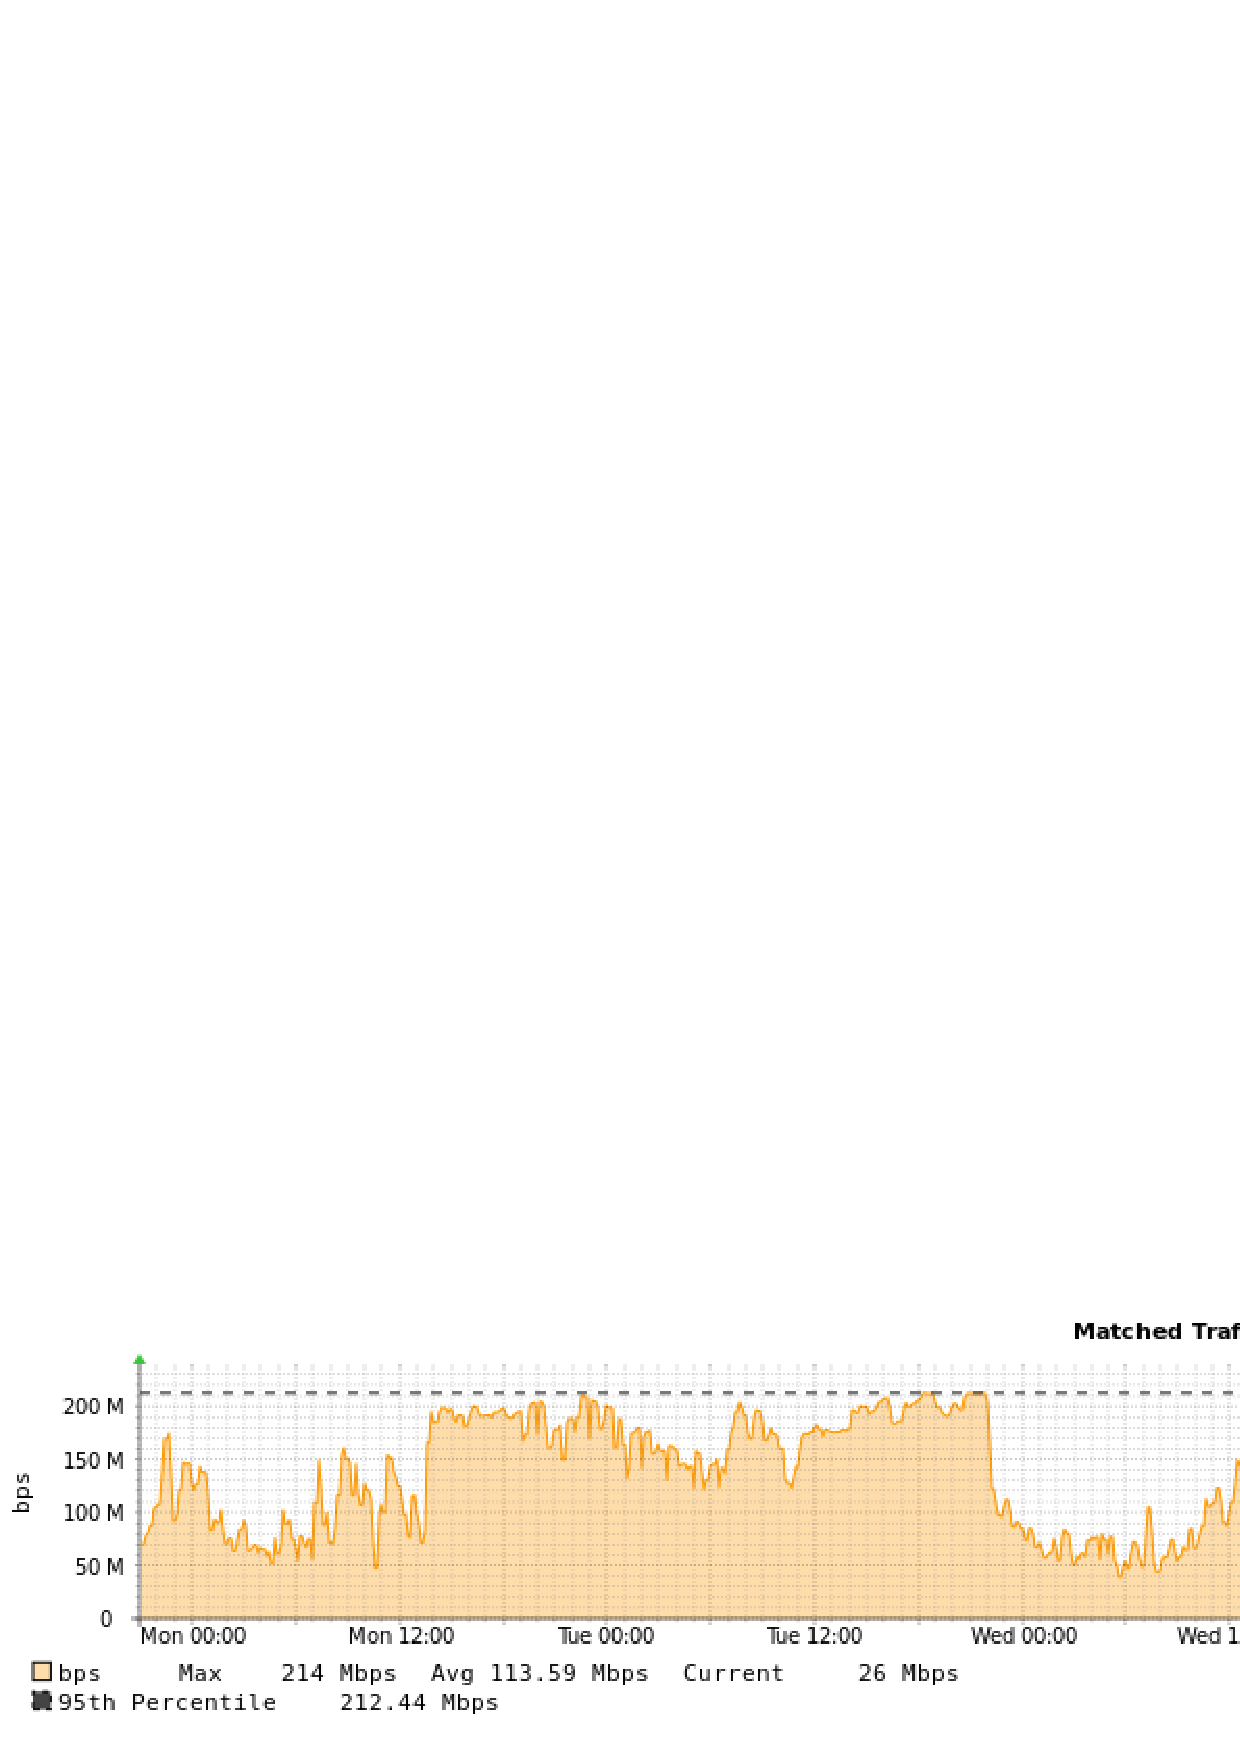
\includegraphics[scale=0.1]{..\images\wacsinmidjun.pdf}
The number of concurrent jobs is limited to 1500 to try to balance the network 
starvation while having as high job count as possible. When we tried to up this count to 1800 of the available 2400 the error rate spiked to 6000 failed jobs in 24 hours
from the usual average of 500.
.

\subsection{Storage}
Although the original spec called for 400TB for each experiment, after the reconfiguration of the storage due to 
inherent failures of raid5 arrays with 30 disks, this has now been reduced to 348 TB for ALICE and 258 TB for ATLAS.
ATLAS was supposed to get an additional 100TB from the original storage we had before the new hardware but that has 
proven to not with stand tests. ATLAS will however be equal to ALICE in storage volume when all the new storage 
is finalised and goes live.

\subsection{Monitoring}
We are monitored by numerous parties, from WLCG, EGI, ALICE experiment, ATLAS experiment, and of course
ourselves. Our local monitoring system is a zabbix 2.4 (http://zabbix.com) setup with grafana (http://grafana.org) for dashboards. In the interests of transparency
the grafana dashboards are bing made public and zabbix will be opened to the HEP community via federated logins.\\
The monitoring extends from the basic hardware information and triggers for temperature, cpu load, etc. all the way up to 
job states,  processing efficiency, and network utilisation.

\subsection{Africa Arabia Regional Operations Centre} 
We fall under the AAROC region, and together with them we have our software and ticketing system on github.com/AAROC
This is all done in the interests of transparency, and collaboration. The ticketing system is under www.github.com/AAROC/chpctier2
as is the source code for the configuration of our site and various other sites in the operations centre.
Our code for configuration management and shortly the analysis facility is also there allowing other to contribute and 
collaborate with us, and for us to put something back.

\subsection{Incidents}
In the 4 months since I started various problems have occurred.
\begin{itemize}
  \item 17 March a switch dies, killing everything, down for 4 days due to next business day support.\\
    Point of failure removed and network restructured to harness the redundancy of the 10Gbps network.
  \item 14 April dead disk , 15 April new disk arrives, 16 April rebuild fails, 109TB of RAID5 storage lost.
  \item 21 May Power upgrade to site, down from Friday to Monday.
  \item 22 June General power failure (c. 1 hour), generator failed to start, storage out for 2 days.
\end{itemize}

\subsubsection{Bandwidth}
Since starting on 1 March we have progressively cleaned up the ALICE operations to the point of almost
all error jobs are now user related or network related. This has meant that we are now very regularly consuming all our
bandwidth incoming and outgoing. The result of this is large scale job failures when the bandwidth starvation lasts for too long.
We currently have 212Mbps incoming and outgoing. 
\begin{figure}
\begin{center}
  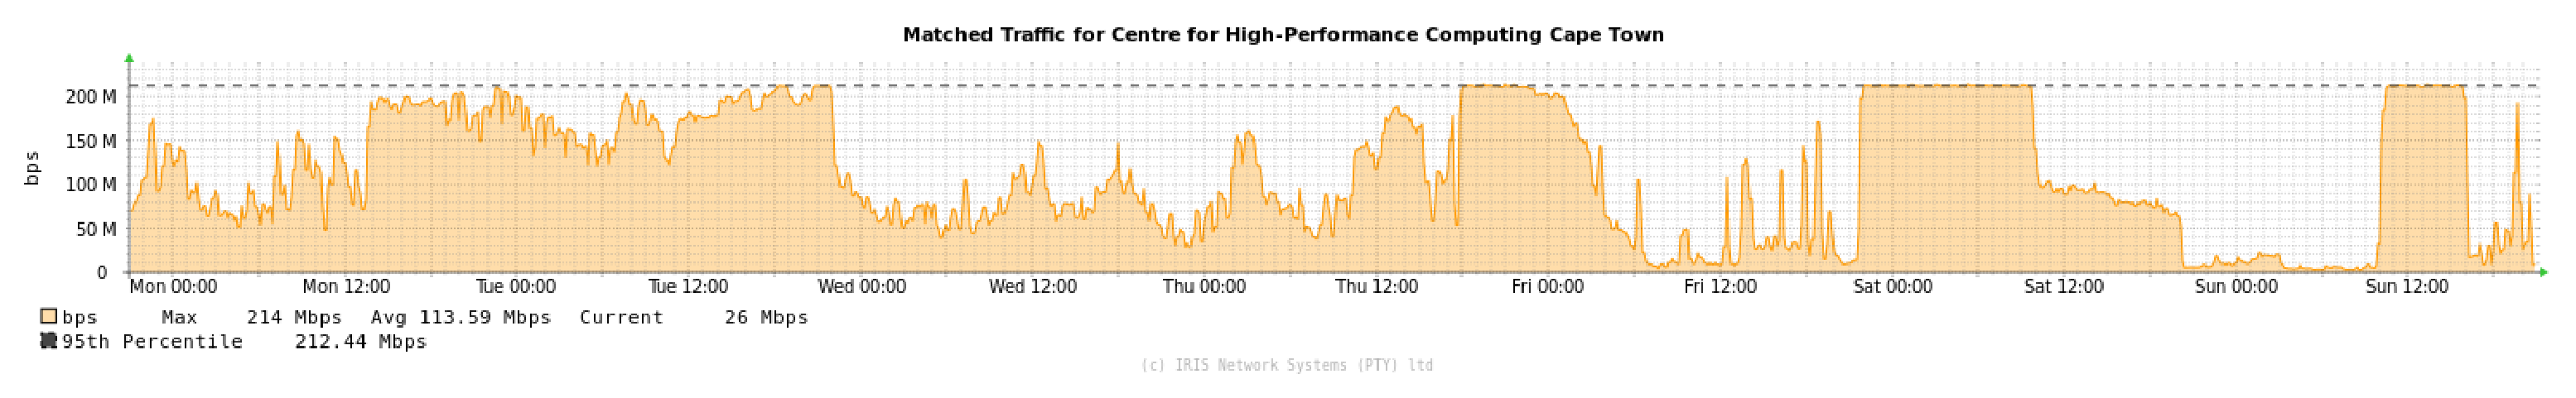
\includegraphics[width=38pc]{wacsinmidjun.eps}
  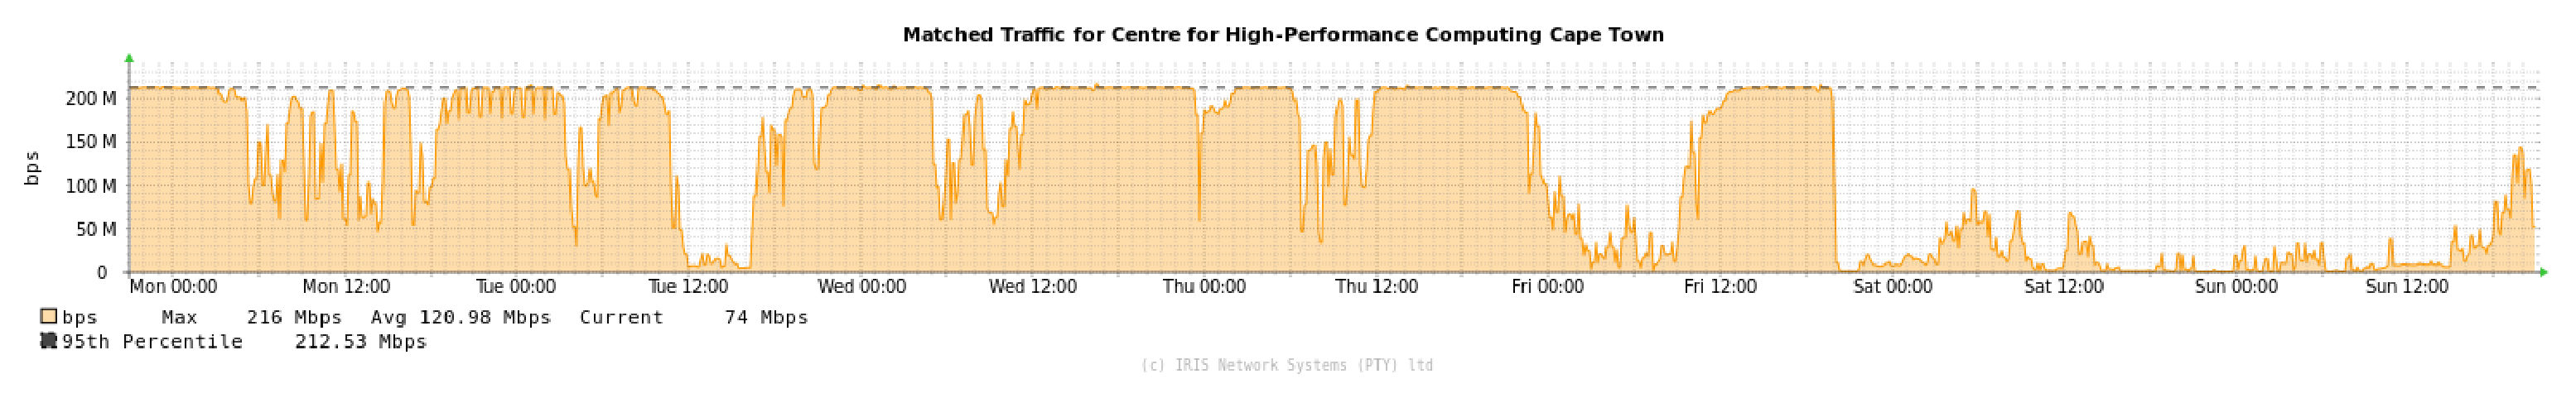
\includegraphics[width=38pc]{seacomoutmidjun.eps}
\end{center}
\caption{\label{label}Bandwidth utilisation of C.H.P.C. for international traffic. Upper graph is incoming, and the lower one is outgoing. This is for the second week of June and shows the clear flat lining of the data, which then causes job to starve either for incoming data or writing their outputs.}
\end{figure}
The bandwidth 
%\begin{figure}[h]
%    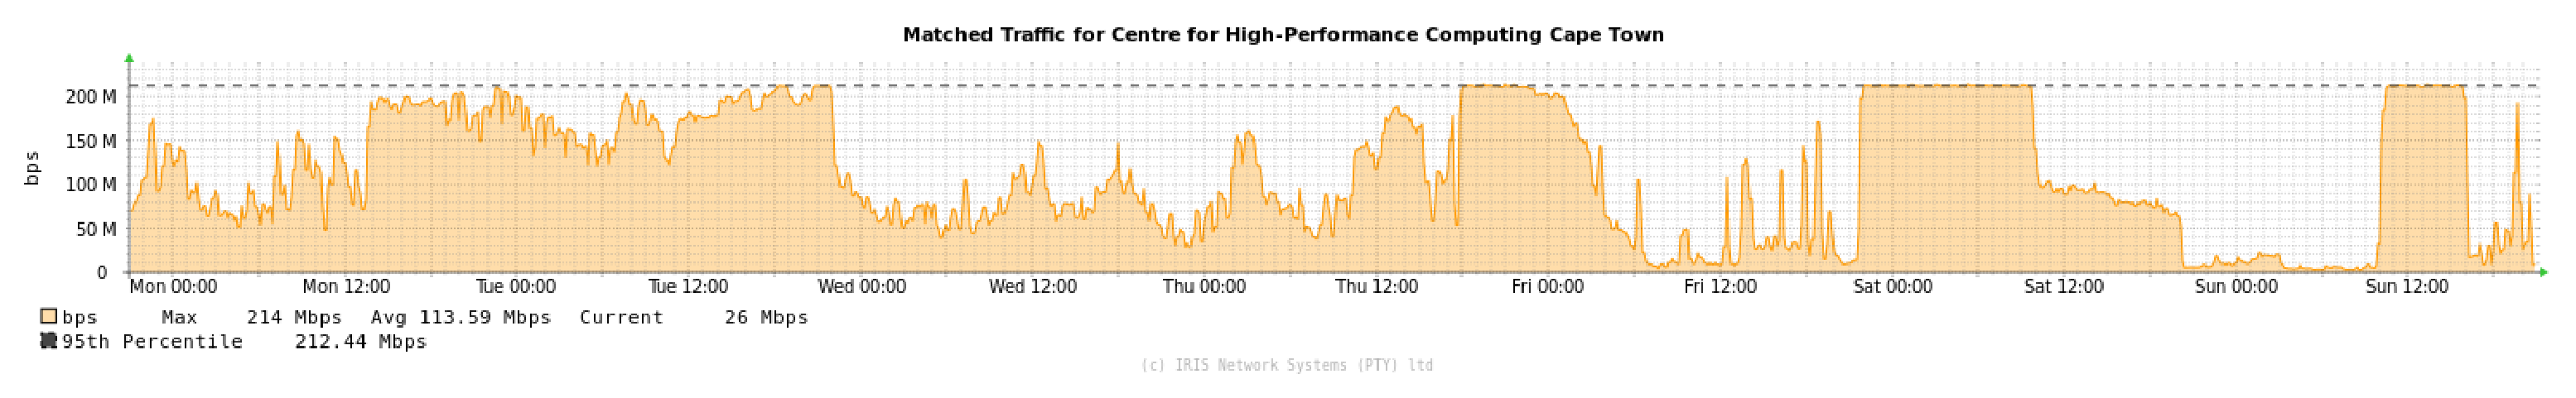
\includegraphics[width=38pc]{wacsinmidjun.eps}
%    \caption{\label{label}Figure caption for first of two sided figures.}
%\end{figure}
%\begin{figure}[h]
%    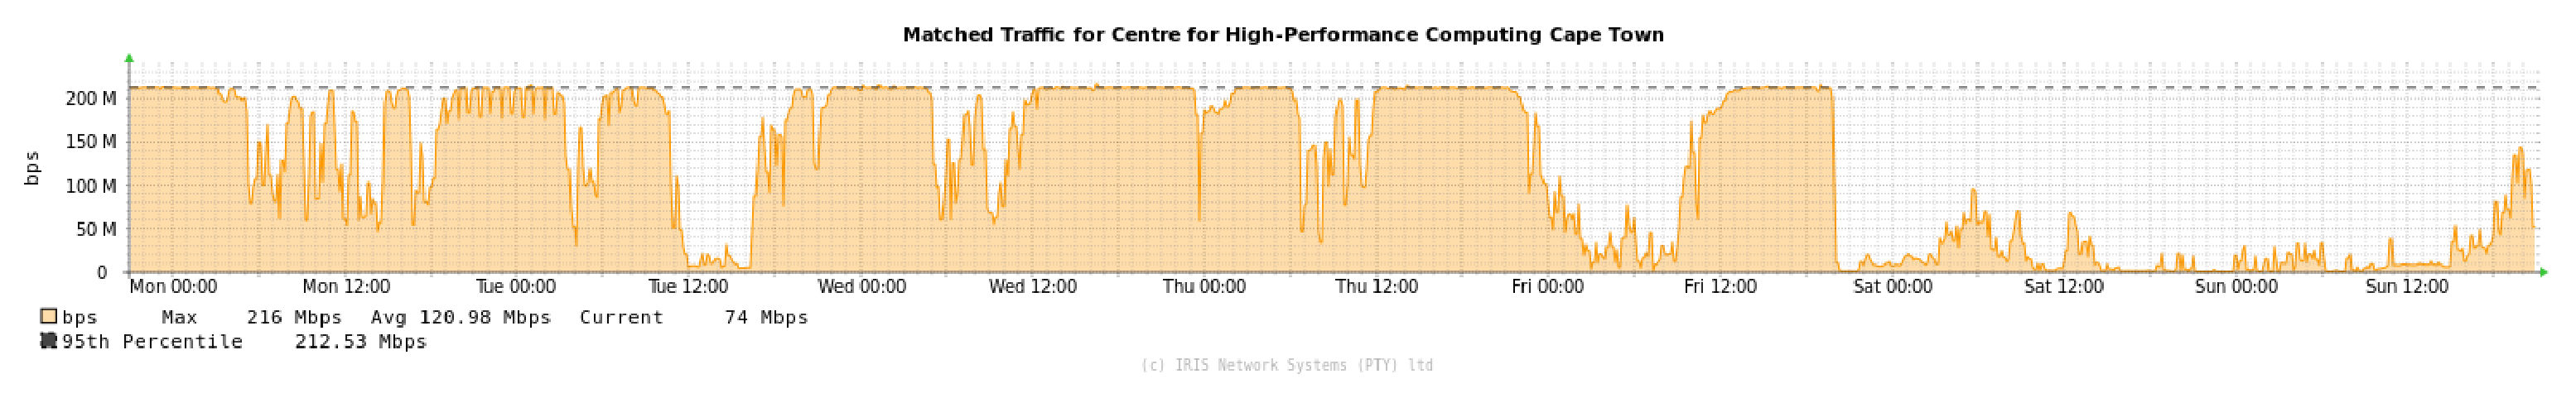
\includegraphics[width=38pc]{seacomoutmidjun.eps}
%    \caption{\label{label}Figure caption for second of two sided figures.}
%\end{figure}



%\begin{figure}
% 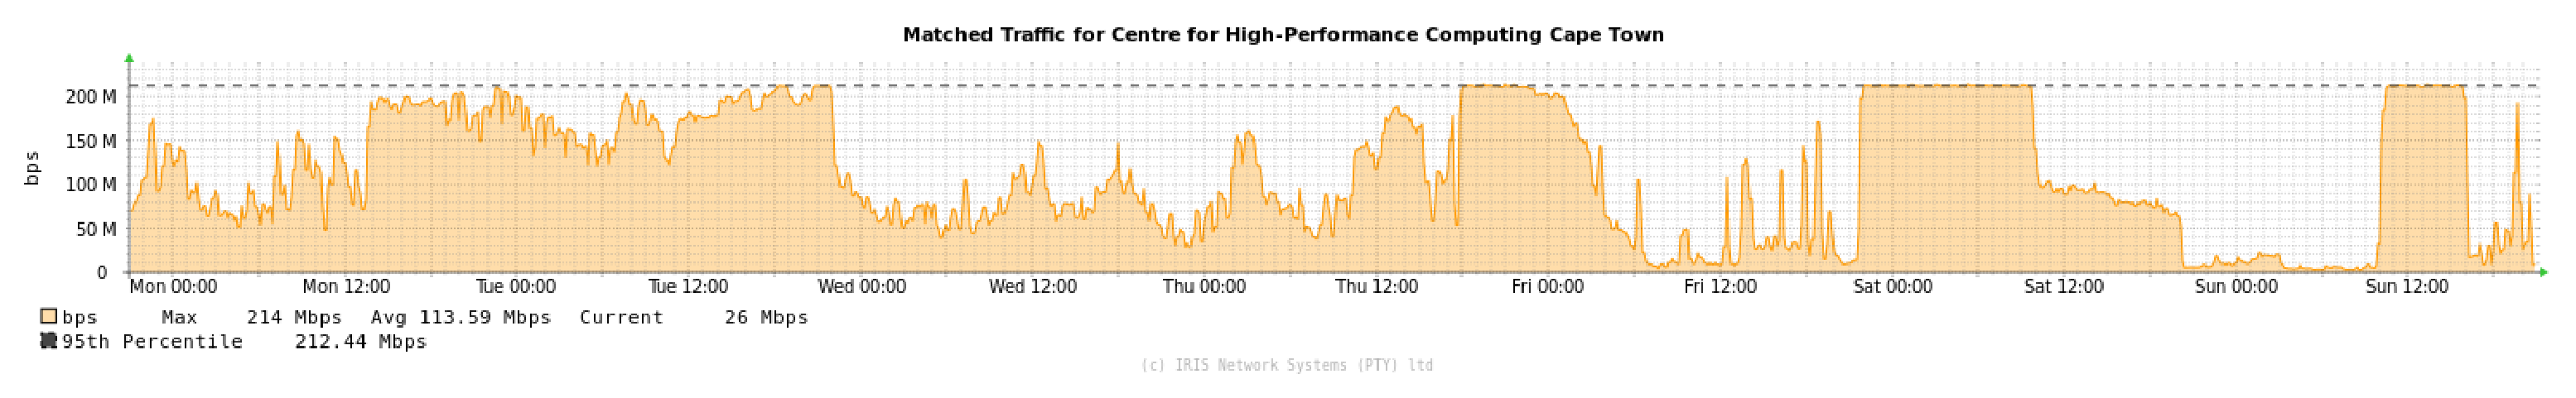
\includegraphics[scale=0.4]{wacsinmidjun.eps}
%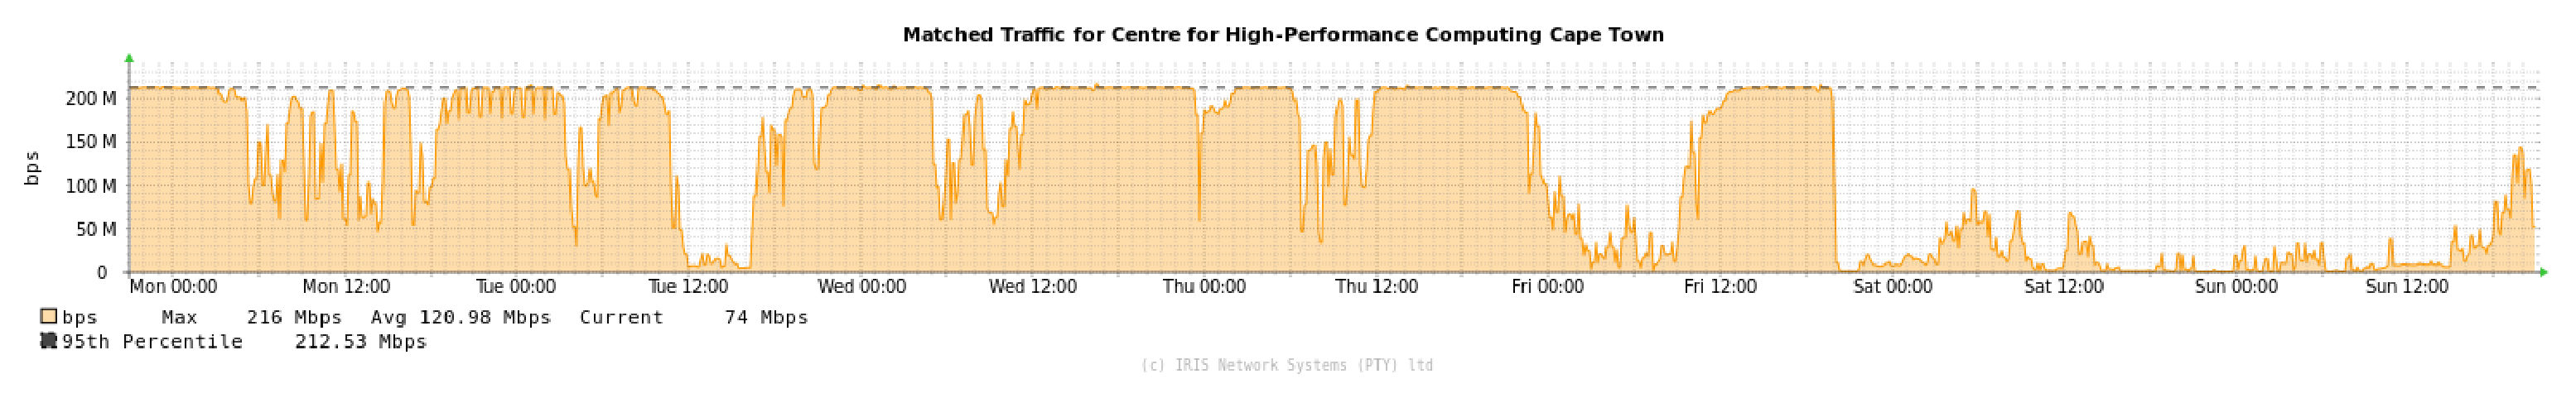
\includegraphics[scale=0.4]{seacomoutmidjun.eps}
%\end{figure}

\section{User Analysis}
The 34 nodes are to be reconstituted into an analysis facility and general facility for 
South African Grid virtual organisation. They were recently redeployed back to HEP. This will provide the domestic Physics community 
the ability to do local analisys and Monte Carlo as they see fit. 
These nodes are to be configured differently from the Tier2 nodes as these will all be containerised in the upgrades.
All software will come from CVMFS via CODE-RADE (http://github.com/AAROC/CODE-RADE), or from users prepackaging their code and its dependencies inside their submissions.
This part of the site will be more tightly integrated with AAROC, and as such, Fermionic Molecular Dynamics has been ported for use via CODE-RADE, with more to applications
specific to physics to come.

This is with a view to eventually making the Tier2 site virtual with containers as well, once the 34 are stable and operating properly later on.
\subsection{Upgrades}
Since starting at C.H.P.C. it became clear that the entire system needed a reinstall due to instabilities. It was hoped to postpone this until
CentOS7 was approved and validated for use and then do everything at once. We can no longer keep postponing this, but we need to keep our system running as 
much as possible to keep our availability and reliability up.\\

The current planned upgrade strategy to achieve more stability, be Tier2 compliant and create greater clarity for external users is :
\begin{itemize}
  \item Reconfigure all storage to smaller raid6 arrays (completed). This was in lieu of failures.
  \item Redo all network for redundancy.
  \item Reinstall/upgrade all cluster, both parts. 
  \item Implement configuration management, puppet in our case.
  \item Acquire more storage to make us compliant for ALICE and ATLAS Tier2, and additional storage for the user analysis facility.
  \item Virtualise the management servers to remove their underlying hardware as points of failure, they can migrate in the case of hardware failure.
  \item Open up the monitoring and ticketing systems for all to see to be completely transparent.
  \item Expand the monitoring for more in depth application specific knowledge.
  \item Extend the bandwidth to improve our efficiency and use all the available cpu slots.
\end{itemize}
 

\section{Conclusion and planning ahead}
The facility has been operating with some impediments but currently runs 1500 ALICE concurrently with very few error caused by the site.
In the coming year we plan to map out a path to tier1 status. To achieve this the site needs to be more stable, and predictable. 
A complete reinstall is currently being tested and the upgrades listed earlier should get us to a more stable situation and able to achieve the 95\% uptime expected of a tier2.
The intended additional bandwidth and storage will make us Tier2 compliant.

\end{document}


